%; whizzy chapter
% -initex iniptex -latex platex -format platex -bibtex jbibtex -fmt fmt
% $B0J>e(B whizzytex $B$r;HMQ$9$k>l9g$N@_Dj!#(B

%     Kansai Debian Meeting resources
%     Copyright (C) 2007 Takaya Yamashita
%     Thank you for Tokyo Debian Meeting resources

%     This program is free software; you can redistribute it and/or modify
%     it under the terms of the GNU General Public License as published by
%     the Free Software Foundation; either version 2 of the License, or
%     (at your option) any later version.

%     This program is distributed in the hope that it will be useful,
%     but WITHOUT ANY WARRANTY; without even the implied warranty of
%     MERCHANTABILITY or FITNESS FOR A PARTICULAR PURPOSE.  See the
%     GNU General Public License for more details.

%     You should have received a copy of the GNU General Public License
%     along with this program; if not, write to the Free Software
%     Foundation, Inc., 51 Franklin St, Fifth Floor, Boston, MA  02110-1301 USA

%  preview (shell-command (concat "evince " (replace-regexp-in-string "tex$" "pdf"(buffer-file-name)) "&"))
% $B2hA|%U%!%$%k$r=hM}$9$k$?$a$K$O(Bebb$B$rMxMQ$7$F(Bboundingbox$B$r:n@.!#(B
%(shell-command "cd image200708; ebb *.png")

%%$B$3$3$+$i%X%C%@3+;O!#(B

\documentclass[mingoth,a4paper]{jsarticle}
\usepackage{kansaimonthlyreport}
\usepackage{ascmac}

% $BF|IU$rDj5A$9$k!"Kh7nJQ$o$j$^$9!#(B
\newcommand{\debmtgyear}{2008}
\newcommand{\debmtgdate}{23}
\newcommand{\debmtgmonth}{2}
\newcommand{\debmtgnumber}{10}

\begin{document}

\begin{titlepage}

% $BKh7nJQ99$9$kItJ,(B, $BK\J8$NKvHx$b=$@5$9$k$3$H$r$o$9$l$:$K(B

 $BBh(B\debmtgnumber{}$B2s(B $B4X@>(B Debian $BJY6/2q;qNA(B

\vspace{2cm}

\begin{center}
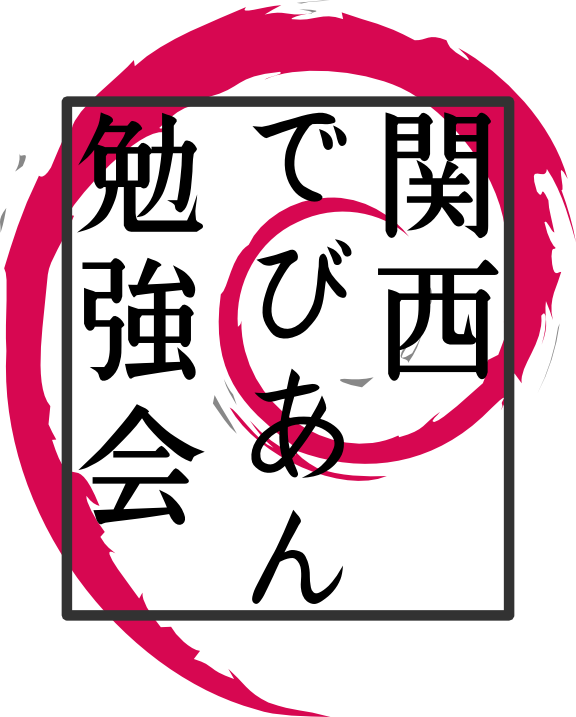
\includegraphics{image200802/kansaidebianlogo.png}
\end{center}

\begin{flushright}
\hfill{}$B4X@>(B Debian $BJY6/2qC4Ev<T(B $B;32<(B $BB:Li(B\\
\hfill{}\debmtgyear{}$BG/(B\debmtgmonth{}$B7n(B\debmtgdate{}$BF|(B
\end{flushright}

\thispagestyle{empty}
\end{titlepage}

\dancersection{Introduction}{$B;32<(B $BB:Li(B}
 
 $B4X@>(B Debian $BJY6/2q$O(BDebian GNU/Linux $B$N$5$^$6(B
 $B$^$J%H%T%C%/(B($B?7$7$$%Q%C%1!<%8!"(BDebian $BFCM-$N5!G=$N;EAH!"(BDebian $B3&7($G5/(B
 $B$3$C$?=PMh;v!"$J$I$J$I!K$K$D$$$FOC$79g$&2q$G$9!#(B

 $BL\E*$H$7$F<!$N;0$D$r9M$($F$$$^$9!#(B
 \begin{itemize}
  \item ML$B$d7G<(HD$G$O$J$/!"D>@\4i$r9g$o$;$k;v$G$N>pJs8r49$NB%?J(B
  \item $BDj4|E*$K=8$^$l$k>l=j(B
  \item $B;qNA$N:n@.(B
 \end{itemize}

 $B$=$l$G$O!"3Z$7$$0l;~$r$*3Z$7$_2<$5$$!#(B

\newpage

\begin{minipage}[b]{0.2\hsize}
 {\rotatebox{90}{\fontsize{80}{80}
{\gt $B4X@>%G%S%"%sJY6/2q(B}}}
\end{minipage}
\begin{minipage}[b]{0.8\hsize}
\hrule
\vspace{2mm}
\hrule
\setcounter{tocdepth}{1}
\tableofcontents
\vspace{2mm}
\hrule
\end{minipage}

\dancersection{GIS on Debian GNU/Linux!}{$B@6Ln(B $BM[0l(B}

\subsection{$B$O$8$a$K(B}
\subsubsection{$B<R2qE*@0Hw$N?JE8(B}

\begin{itemize}
 \item $B9q:]>p@*(B
       \begin{itemize}
	\item $BCO?^>pJs$rEE;R2=$7$F07$*$&$H$$$&;n$_$O(B1960$BG/Be$4$m$+$i;O$^$C$F$$(B
	      $B$k!#Ev=i$O8&5fL\E*!#(B
	\item $B%a%$%s%U%l!<%`>e$G$O$J$/!"%o!<%/%9%F!<%7%g%s$d%Q!<%=%J%k%3%s%T%e!<(B
	      $B%?$NH/C#$KH<$$!"(B1980$BG/Be:"$+$i$3$l$i$N%3%s%T%e!<%?>e$GF0$+$;$k%7(B
	      $B%9%F%`$,Ia5Z$7;O$a$k!#(B
	\item $B8e=R$9$kCO>e4QB,1R@1!J%i%s%I%5%C%H1R@1(B1$B9f5!$NBG$A>e$2$O(B1972$BG/!K$d(B
	      $B%9%Z!<%9%7%c%H%k$N1?MQ$K$h$j!"%j%b!<%H%;%s%7%s%0$J$I$N3hMQ$,(B1970
	      $BG/Be$h$j9T$o$l$k$h$&$K$J$k!#(B
       \end{itemize}
 \item $BF|K\9qFb(B
 \begin{itemize}
  \item $B9T@/%5%$%I(B \\
	$BF|K\$K$*$$$F$O!"9qEZ$K4X$9$k?tCM>pJs$NEE;R2=(B
	\begin{quotation}
	 $B!VJ?@.(B7$BG/(B1$B7n$N:e?@!&(B
	 $BC8O)Bg?L:R$NH?>JEy$r$-$C$+$1$K!"@/I\$K$*$$$F!"(BGIS$B$K4X$9$kK\3JE*$J(B
	 $B<hAH$,;O$^$C$?!#!W!J9qEZCOM}1!(B
	 GIS\footnote{\url{http://www.gsi.go.jp/GIS/whatisgis.html}}$B$K$h$k!K(B 
	\end{quotation}
	$B"*9q$r5s$2$F$N@/:v<B;\!#(B2002$BG/$N>.@tFb3U$K$*$1$k!V(Be-Japan$B=EE@7W(B
	$B2h(B-2002$B!W$N=EE@@/:v$N$&$A!"(B4$BHVL\$N!V9T@/$N>pJs2=5Z$S8x6&J,Ln$K$*(B
	$B$1$k>pJsDL?.5;=Q$N3hMQ$N?d?J!W$K$*$$$F(BGIS$B$N?d?J$,@9$j9~$^$l$k!#(B
	ex)$B9qEZCOM}1!$N?tCMCO?^(B(CD-ROM$BHG(B)$B$OJ?@.(B9(1997)$BG/:"$+$i@0Hw$5$l$k(B
	$B$h$&$K$J$C$F$-$F$$$k!#(B
  \item $B7z@_%5%$%I(B
	\begin{itemize}
	 \item CAD(Computer Aided Design)$B$NIa5Z(B
	 \item $BEE;RG<IJ!&I8=`2=(B
	 \item $B7z@_>J!&9qEZ8rDL>J$N8e2!$7(B
	\end{itemize}
 \end{itemize}
\end{itemize}

\subsubsection{$B8D?M%l%Y%k(B}
\begin{itemize}
 \item Google Earth$B!"(BNASA World Wind$B$J$I$NL5NA$+$D9b@-G=$J%G%9%/%H%C%WCO(B
       $B?^%S%e!<%o!<$NEP>l(B \\
       $B"*(B"Google Earth$B%7%g%C%/(B"
 \item Google Map$B$J$I$N(BWeb$B%^%C%T%s%0%5%$%H(B \\
       $B"*(BMashUp$B$,N.9T(B\\
       $B"*6u4V>pJs$r8D?M$,07$&;~Be$K!#(B
\end{itemize}

\subsection{GIS$B$H$O(B}
\subsubsection{$BDj5A(B}
\begin{itemize}
 \item $B9qEZCOM}1!(B\footnote{\url{http://www.gsi.go.jp/GIS/whatisgis.html}}$B$N@bL@(B
       \begin{quotation}
	$BCOM}>pJs%7%9%F%`!J(BGIS$B!'(BGeographic Information System$B!K$O!"COM}E*0LCV$r<j$,$+$j$K!"0LCV$K4X$9$k(B
	$B>pJs$r;}$C$?%G!<%?!J6u4V%G!<%?!K$rAm9gE*$K4IM}!&2C9)$7!";k3PE*$KI=<($7!"9bEY$JJ,@O$d?WB.$JH=CG(B
	$B$r2DG=$K$9$k5;=Q$G$"$k!#(B 
       \end{quotation}
 \item GIS$B%]!<%?%k%5%$%H(B
       \footnote{\url{http://www.gis.go.jp/contents/about/whatis/index.html}}$B$N@b(B
       $BL@(B
       \begin{quotation}
	GIS$B!J(BGeographic Information System$B!'COM}>pJs%7%9%F%`!K$H$O!"0LCV$d6u4V$K4X$9$kMM!9$J>pJs$r!"%3(B
	$B%s%T%e!<%?$rMQ$$$F=E$M9g$o$;!">pJs$NJ,@O!&2r@O$r$*$3$J$C$?$j!">pJs$r;k3PE*$KI=<($5$;$k%7%9%F%`(B
	$B$G$9!#85!9$O@lLgE*$JJ,Ln$G$NMxMQ$,0lHLE*$G$7$?$,!":G6a$G$O!";d$?$A$N@83h$NCf$G$N?H6a$JMxMQ$X$H(B
	$B!"$=$N3hMQHO0O$,9-$,$C$F$-$F$$$^$9!#(B 
       \end{quotation}
 \item $B9qEZ8rDL>J9qEZ7W2h6I(B
       \footnote{\url{http://www.mlit.go.jp/kokudokeikaku/gis/aboutgis/index.html}}
       $B$N@bL@(B
       \begin{quotation}
	$B0LCV$d6u4V$K4X$9$k>pJs$r$b$C$?%G!<%?!J6u4V%G!<%?!K$rAm9gE*$K4IM}!&2C9)$7!";k3PE*$KI=<($G$-$k9b(B
	$BEY$JJ,@O$d?WB.$JH=CG$r2DG=$K$9$k5;=Q$G$9!#(B 
       \end{quotation}
 \item ESRI$B%8%c%Q%s<R(B
       \footnote{\url{http://www.esrij.com/whatisgis/gis/index.shtml}}$B$N@bL@(B
       \begin{quotation}
	GIS$B$H$O!"(BGeographic Information System$B$NN,$G!"9-5A$K$O!V<B@$3&$r6u4VE*$K4IM}$9$k$3$H$K$h$j(B
	$B!"$h$j9gM}E*$J0U;W7hDj$r9T$*$&$H$9$k%"%W%m!<%AA4HL!W$r0UL#$7$^$9$,!"695A$K$O!"!V6u4V>pJs$r:n@.(B
	$B!"2C9)!"4IM}!"J,@O!"I=8=!"6&M-$9$k$?$a$N>pJs%F%/%N%m%8!W$r0UL#$7$^$9!#(B 
       \end{quotation}
 \item $B%$%s%U%)%^%F%#%/%9<R(B
       \footnote{\url{http://www.informatix.co.jp/sis/aboutgis/aboutgis.html}}$B$N(B
       $B@bL@(B
       \begin{quotation}
	GIS$B$H$O!"(BGeographical Information Systems$B!JCOM}>pJs%7%9%F%`!K$NN,$GCO?^>e$KMM!9$J>pJs$r=E$M(B
	$B9g$o$;$FI=<(!&JT=8$7$?$j!"J,@O$9$k%7%9%F%`$N$3$H$r$$$$$^$9!#(B
       \end{quotation}
\end{itemize}

\begin{itembox}[c]{"GIS"$B$H(B"GPS"$B$N0c$$$C$F$o$+$k!)(B}
$B:.F1$7$F$$$k?M$rNI$/8+$+$1$^$9!#(BGPS="Global Positioning System"$B$NN,!#(B

$BA4CO5eB,0L%7%9%F%`!"HFCO5eB,0L%7%9%F%`!#%"%a%j%+$N1R@1%7%9%F%`!#8573;vMQ!#(B

$B%+!<%J%S$H$+7HBSEEOC$KF~$C$F$$$k%d%D$M!#(B
\end{itembox}

\subsubsection{$BBgJL$7$F(B2$B%?%$%W(B}
\begin{itemize}
 \item $B4IM}7O(BGIS
       \begin{itemize}
	\item $BE}9g7?!&A4D#7?(B \\
	      $B>&MQ@=IJ$,<gN.!#%i!<%8%9%1!<%k;X8~!#J,@O$b=PMh$k!#(B\\
	      $B"*(BESRI$B<R(BArcGIS$B!"%$%s%U%)%^%F%#%/%9<R$N(BSIS$B!"(BMapInfo$B<R$N(BMapInfo$B$J$I!#(B
	      \\
	      $B"*<B:]!"=u@.6b$J$I$G$*6b$,$"$k?M$O!"8D?M8&5f<T$G$bF3F~$9$k?M$OB?(B
	      $B$$!#(B\\
	      $B"*$=$N>l9g!"A`:nJ}K!$rCN$C$F$$$k$3$H$G="?&;~$N%"%I%P%s%F!<%8$K$b!#(B
	\item $BI=<(7O!'(BGoogle Earth$B!"(BGoogle Map$B$_$?$$$J%b%N!#(B
	\begin{itemize}
	 \item mapserver:WebGIS$B%5!<%P(B
	       \footnote{\url{http://mapserver.gis.umn.edu/}}
	 \item ka-Map\footnote{\url{http://ka-map.maptools.org/}}
	\end{itemize}
	\item CAD$B$H$N4X78(B\\
	      $B@_7W!&B,NL!&7z@_!&EZLZ!&KI:R$HL)@\$KO"7H(B\\
	      $B"*6-L\$,[#Kf$K$J$C$F$-$F$$$k(B\\
	      $B"*(BAutodesk(AutoCAD)$B<R$N%*!<%W%s%=!<%9$X$N;2F~(B
       \end{itemize}
 \item $B2r@O7O(BGIS
       \begin{itemize}
	\item GRASS GIS\footnote{\url{http://grass.itc.it/}}\\
	      1980$BG/BeH>$P$+$i3+H/(B
	\item Quantum GIS\footnote{\url{http://www.qgis.org/}}\\
	      $B9b5!G=$J%S%e!<%o!#4JC1$J2r@O5!G=$b;}$D!#(B
	\item SAGA
	      GIS\footnote{\url{http://www.saga-gis.uni-goettingen.de/html/index.php}}\\
	      Release 2.0.1$B$O(BGentoo Linux$B$N(BPortage$BMQ$,MQ0U$5$l$F$k$_(B
	      $B$?$$!#(B
	\item Mandara\footnote{\url{http://www5c.biglobe.ne.jp/~mandara/}}\\
	      Windows$BMQ$N(BGIS$B%=%U%H!#=i?4<T8~$1!#(BGIS$B$,$I$&$$$&$b$N$+$r$F$C$H$jAa(B
	      $B$/CN$j$?$$?M$K$O$*<j7Z$+$b!#(BMS Excel$B$H$NO"7H$b!#(B
       \end{itemize}
\end{itemize}

\subsection{$B:G6a$NOCBj(B}
\begin{itemize}
 \item OSGeo$B:bCD(B\footnote{\url{http://www.osgeo.org/node/271}}$BF|K\;YIt(B\footnote{\url{http://www.osgeo.jp/}}\\
       $BBg:e;TN)Bg3X$d3t<02q<R%*!<%/%K!<$J$I$,Cf?4(B
 \item $B4X@>%*!<%W%s%=!<%9(B2007$B$K$*$1$k%+%s%U%!%l%s%9(B\footnote{\url{http://www.osgeo.jp/?page_id=8}}\\
       $B!VFCJL4k2h!'(BOSGeo.JP$B!!AOB$ET;T$r;Y$($k%*!<%W%s%=!<%9(B GIS$B$N:GA0@~!W(B
 \item $B=q@R$N@0Hw(B
       \begin{itemize}
	\item $B!XF~Lg(BWeb$B%^%C%T%s%0!J(B\textit{Web Mapping Illustrated}$B!K!Y(B(2006$BG/(B5$B7n!"(B
	      $B%*%i%$%j!<(B)\footnote{\url{http://www.oreilly.co.jp/books/4873112826/}}
	\item \textit{Open Source Gis: A Grass Gis Approach}(2007$BG/Kv$K(B3rd
	      Edition$B$,=P$?!"(BSpringer)\footnote{\url{http://www.grassbook.org/}}
       \end{itemize}
\end{itemize}

\subsection{$B$J$<(BDebian GNU/Linux$B$+!)(B}
\subsubsection{Debian GNU/Linux$B$rA*$s$@F15!(B($B8D?ME*7P83(B)}
\begin{itemize}
 \item[$B!z(B] $B%*!<%W%s%=!<%9$J%=%U%H%&%'%"$,;H$$$?$+$C$?!#(B\\
       $B"*9b5!G=$J%W%m%W%i%$%(%?%j$J%=%U%H%&%'%"$OBt;3$"$k$,!"9b2A!*AH?%$dJd=u6b$GF3F~$7$?>l9g(B
	   $B$O%i%$%;%s%9$NLdBj$,(B$\dots$$B!#(B\\
	$B"*%W%m%0%i%^%V%k$J$N$b$$$$$+$b(B($BJY6/$K$J$k$+$b(B)
 \item[$B!z(B] DebianGIS$B$N$h$&$J%W%m%8%'%/%H$,$"$k!J:G6a$ODdBZ5$L#!)!K(B
 \item[$B!{(B] $B=i?4<TE*$K!"%Q%C%1!<%8$N4IM}$,3Z$=$&$@$C$?(B(APT$BK|:P(B!!)$B!#(B
 \item[$B!|(B] $B$G$b!";H$$$3$J$;$k$J$iB>$N%G%#%9%H%j%S%e!<%7%g%s$G$b(BOK$B!)(B\\
	   $B"*%=!<%9%3!<%I$O8x3+$5$l$F$k$3$H$,B?$$$7!"(BDebian GNU/Linux$B$8$c(B
	   $B$J$-$c%@%a$J%P%$%J%j$H$$$&$N$OL5$$$H;W$&!#(B\\
	   $B"*(BWindows$B>e$G;H$($k4D6-$bCe!9$H?J$s$G$-$F$$$k!#$^$@(BUnix/Linux
	   $B$K%"%I%P%s%F!<%8$,$"$k$1$I!#(B\\
	   $B"*(BMacOS$B$O(BGIS$B$O$"$s$^$jF@0U$8$c$J$$$+$b(B$\dots$$B!#(B
 \item[$B!|(B] $B3$30$G$O(BMandriva$B$H$+(B($B$+$D$F$N(BArcheOS$B$H$+(B)Gentoo
	   Linux(Gentoo-GIS overlay Project \footnote{\url{http://gentoo-gis.sourceforge.net/}}$B$J$s$F$N(B
	   $B$,$"$k!#(B)$B$J$I$b$h$/MxMQ$5$l$F$$$kLOMM!#(B
 \item[$B!|(B] $B:G6a$O?M$K4+$a$k$H$7$?$i(BUbuntu$B$+(B$\dots$$B!#(B($B8D?ME*$K>R2p<B@SM-$j(B($B5c(B))
\end{itemize}

\subsubsection{Debian GNU/Linux$B$K$*$1$k%Q%C%1!<%8!"%i%$%V%i%j$J$I(B}

DebianGIS\footnote{\url{http://wiki.debian.org/DebianGis}}$B$N%j%9%H$+$i(B

\begin{commandline}
Geospatial packages of core concern
    Meta-packages
        *education-geography task from debian-edu: DebianGIS recommends these additions: qgis, gmt, gdal, proj.
 (education-geography already depends on grass):
    Binary packages
        *PostGIS
            RDBMS$B$N(BPostgreSQL$B$NCOM}>pJs3HD%(B
        *GDAL(Geospatial Data Abstraction Library $BCOM}6u4V%G!<%?Cj>]2=%i%$%V%i%j!)(B)
            $B:BI87O(B($BEj1F(B)$BJQ49%i%$%V%i%j(B
        *GRASS
        *QuantumGIS. Includes qgis-plugin-grass
        *Mapserver
        *GEOS
        *PROJ: proj-doc: there are PDF files available, perhaps those would be better?
        *Earth3D
        *gpsd
        *gpsdrive
        *gpx2shp
        *gpsman
        *gpsmanshp
        *gpstrans
        *gpsbabel
        *thuban
        *gmt
        *OpenSceneGraph
        *OpenThreads
        *Avce00 and E00compr
        *OGDI
        *OpenJUMP: in debian/contrib, because it depend on batik and sun jre. Work is being done to get batik into 
debian/main, and openjump to work with GNU Classpath. Packaged instead of JUMP
        *JTS
        *TerraLib
        *mapnik
        *marble
        *Viking: a GPS track editor and analyzer
        Useful packages to be packaged
        Sorted by approximate priority.
            Libraries and bindings
            *Python Shapelib binding
            *Python Cartographic Library (PCL)
            *Tcl Shapelib binding
            *Ruby Shapelib binding
        Desktop/Analysis/Database
            *Ossim: currently being worked on (Francesco Lovergine)
            *PostLBS: powerful routing solution for PostgreSQL/PostGIS
            *TerraView: powerful GIS based on TerraLib (already in Debian, but obsolete)
            *OpenModeller: species occurrence modelling software
            *r-spatial: R/GRASS interface for GRASS 6 and other spatial software for R
                R$B8@8l(B:$BE}7W=hM}!#6u4VE}7W%i%$%V%i%j(B
            *garmin-utils: similar in scope and function to gpstrans, but works with modern serial Garmins. 
See also the NetBSD port
            *e-foto: aerial photogrammetry. See this unanswered post
        Data
        OpenStreetMap
            *OpenStreetmap: Useful for upcoming release of gpsdrive
            *josm: Java Open Street Map Editor
            *gosmore: viewer of OSM XML data such as the planet.osm
        Sample datasets
            * GRASS's Spearfish dataset
            * OSGeo's NC sample dataset
    Java
        *gvSIG (top priority)
        *uDig: User-friendly Desktop Internet GIS
        *GeoServer
        *Postgisdriver-JUMP: currently being worked on. Contrib - depends on jump
        *GeoTools: Java GIS Toolkit
        *Deegree2 and iGeoPortal: currently being worked on. Binary package structure not yet clear.
        *NASA World Wind (Java version): Needs JOGL and perhaps SUN Java
        *JOGL: Java
        *Kosmos Desktop GIS derived from OpenJUMP (an unofficial package available)
            For more info on the Java state in Debian, see the moving java to Debian/main page.
    Live Web Apps
        *PyWPS: Python Web Processing Service
        *OpenLayers, TileCache, FeatureServer (all from MetaCarta)
        *p.mapper (unofficial packages available
    3D Visualization
        *ParaView: Very useful for 3D rapresentation of GRASS rasters and vectors
        *Visual Terrain Project: proposed
        *VisIt: 3D visualization
        *X3D: modern version of VRML, various libs & apps
        *OpenDX: the open source version of IBM's Visualization Data Explorer. Uses the IBM Public License
        *MINI: proposed, needed for VTerrain
        *OpenProducer: proposed, useful for OpenSceneGraph
    Lower Priority
        *Shape file utilities, including ShapeChecker
        *http://www.primagis.fi/ map extension for Plone; it builds on top of Mapserver, 
Python Cartographic Library (PCL) and Cartographic Objects for Zope (ZCO)
        *OpenEV: currently being worked on (Alex Bodnaru); old version, based on gtk1; the new one, based on 
gtk2, is still unsuitable to packaging
        *MB-System: multibeam, interferometry, and sidescan sonar data processing (GPL)
        *PhpPgGIS: ITP #381974. Project apparently inactive
        *Open3D GIS: Requires FreeWRL, see http://sourceforge.net/projects/freewrl/.
 Project apparently dead? https://sourceforge.net/projects/open3dgis/
        *dxf2svg: also the reciprocal svg2dxf (depends on pstoedit)
        *JGrass: currently being worked on. Contrib - needs jdk1.4, several contrib packages. Currently being
 fused with uDig - better postpone packaging until settled down
\end{commandline}

$B$3$NB>$K(BFOSS4G Toolkit CD$B$d(BArcheOS(Mandriva$B$@$C$?$,:G6a(BUbuntu$B2=$7$?(B)$B$J$I(B
$B$N(BLive CD$B$b$"$k!#(B\\
$B"*(BFOSS4G Toolkit CD$B$O(BMandriva$B8~$1$N(BRPM$B%;%C%H$H$7$FG[I[$9$k$N$_$H$J$C$?$h(B
$B$&$@!#(B

\subsection{$B6u4V%G!<%?(B}

$B!z0JA0$OI,MW$H$9$k<T$,<+$i<hF@$9$k$3$H$,0lHLE*$G$"$C$?$,!":G6a$G$O3F<o6u4V(B
$B%G!<%?$,@0Hw$5$l$F$-$F$$$k!#(B

\subsubsection{$B9qFb(B}
\begin{itemize}
 \item $B9qEZCOM}1!H/9T$N3F<o?tCMCO?^!JM-=~!K(B\footnote{\url{http://www.gsi.go.jp/}}\\
       $B$?$@$7!"6aG/!">pJs8x3+$K$h$j1\Mw$rL\E*$H$7$F%G!<%?$NL5=~8x3+$,?J(B
       $B$s$G$$$k!#(B\\
       ex)$B9qEZCOM}1!?tCMCO?^(B($B6u4V%G!<%?4pHW(B)$B$N1\Mw!J;n838x3+!K(B
       \footnote{\url{http://sdf.gsi.go.jp/}}
 \item $BEE;R9qEZ%]!<%?%k(B\footnote{\url{http://portal.cyberjapan.jp/index.html}}\\
       $B3F<oCO?^$N1\Mw$r<g4c!#@::Y$J%Y%/%H%k%G!<%?$rDs6!!#@lMQ%W%i%0%$%s(B
       $B$rMQ$$$F3F<+$,(BWeb$BCO?^:n@.$r9T$($k!#(B
 \item $BN&0h4QB,5;=Q1R@1!V$@$$$A!W(B(ALOS)\\
       $B1'Ch9R6u8&5f3+H/5!9=!J(BJAXA\footnote{\url{http://www.jaxa.jp/index_j.html}}$B!K(B
       $B$,(B2006$BG/(B1$B7n(B24$BF|$KBG$A>e$2$?1R@1$N4QB,%G!<%?!#M-NA!)(B
\end{itemize}

$B!V9b@:EY$GI89bCj=P$r9T$&$?$a$N%Q%s%/%m%^%A%C%/N)BN;k%;%s%5(B(PRISM)$B!"$*$h(B
$B$SEZCOHoJ$$N4QB,$r9b@:EY$K9T$&$?$a$N9b@-G=2D;k6a@V30J|<M7W(B2$B7?(B(AVNIR-2)$B!"(B
$BCkLk$NJL$J$/!"$^$?E78u$K$h$i$:N&0h$N4QB,$,2DG=$J%U%'!<%:%I%"%l%$J}<0(BL$B%P(B
$B%s%I9g@.3+8}%l!<%@(B(PALSAR)$B$N(B3$B$D$NCO5e4QB,%;%s%5$rEk:\!W(B

$B"((B2008$BG/(B1$B7n(B8$BF|!"M=Dj$7$?@:EY$,<hF@$G$-$J$$$N$G$O$J$$$+$H$NJsF;(B
\footnote{\url{http://www.asahi.com/special/space/TKY200801090162.html}}
$B$,$J$5$l$?$,!"$=$N8e$ND4::$K$h$j!"F1G/F17n(B16$BF|!"?7$?$JJ}K!$rMQ$$$k$3$H$G7|G0$5$l$F$$$?(B
$BLdBj$O2~A1$G$-$k$H$NH/I=$,$J$5$l$?(B
\footnote{\url{http://www.jaxa.jp/press/2008/01/20080116_sac_daichi_j.html}}$B!#(B

\subsubsection{$BCO5e5,LO(B}
\begin{itemize}
 \item $B%9%Z!<%9%7%c%H%kCO7A%G!<%?(B Shuttle Radar Topography Mission
       (SRTM)\\
       1994$BG/$h$j<B833+;O!#8=:_<g$KMxMQ$5$l$F$$$k$N$O(B2000$BG/$K9T$o$l$?Bh(B3$B2s<B83(B
       $B$K$h$C$F<hF@$5$l$?%G!<%?!#(B11$BF|4V$NHt9T$GN>6K$r=|$/CO>e$NN&CO$NLs(B
       80$B!s!"A4?M8}L)=8CO$NLs(B95$B!s$r%+%P!<$9$k%G!<%?$r<hF@$7$?!#(B

       NASA$B$N(BFTP$B%5%$%H(B\footnote{\url{ftp://e0srp01u.ecs.nasa.gov/srtm/}}$B$h$j%G!<%?$r%@(B
       $B%&%s%m!<%I2DG=!#0lItM-NA!#(B

       DEM(Digital Elevation Model)$B$N:n@.MQ(B
 \item $B%i%s%I%5%C%H1R@12hA|(B Landsat Imagery (TM,
       ETM+)\footnote{\url{http://www.eorc.jaxa.jp/hatoyama/satellite/satdata/landsat_j.html}}\\
       $B%a%j!<%i%s%IBg3X(B
       \footnote{\url{http://glcfapp.umiacs.umd.edu:8080/esdi/index.jsp}}
       $B$+$i%G!<%?$r%@%&%s%m!<%I2DG=!#(B
       $BMM!9$JGHD9$N8w$NH?<M%G!<%?!#%j%b!<%H%;%s%7%s%0MQ!#(B
 \item $B>&MQ1R@12hA|%G!<%?(B\\
       Google Earth$B$d(BGoogle Map$B$J$I$G$O9b@::Y$J>&MQ1R@12hA|%G!<%?$,MQ$$(B
       $B$i$l$F$$$k!#(BEarthsat$B<R$d(BDigital Globe$B<R!"(BBluesky$B<R$J$I!#(B\\
       $B3N$+$K2rA|EY$,9b$/MxMQ2ACM$O9b$$$,!"Hs>o$K9b2A$J$N$G!"HqMQBP8z2L$r9M$($FMxMQ$5$l$F$$$k!#(B
\end{itemize}

$B!z$G$b7k6I8&5fL\E*$N>l9g$J$I$O!":#$G$b<+J,C#$G%G!<%?$r<hF@$7$J$1$l$P$J(B
$B$i$J$$$3$H$NJ}$,B?$$(B($B5c(B)$B!#(B

$B!z$J$N$G!"$$$+$K8zN(E*$K!"I,MW$H$5$l$j@53N!&>\:Y$J6u4V%G!<%?$r<hF@$9$k$+$,LdBj$H$J$k!#(B

\subsection{$B$*$o$j$K(B}
\subsubsection{$B$^$H$a(B}
$B0JA0$KHf$Y$F4D6-$O3JCJ$KNI$/$J$C$F$$$k!#(B

$BFC$K!"$3$A$i$+$iG=F0E*$K3F<o%G!<%?$N@0Hw$rMW5a!&$b$7$/$O<+$iB?Bg$J%3%9%H(B
$B$r$+$1$F<hF@$7$J$/$F$b!"<!!9$H6u4V4pHW%G!<%?$N@0Hw$,9T$o$l$F$-$F$$$k!#(B

$BI=<(7O$NCO?^%5%$%H$J$I$O8D?M%l%Y%k$G4IM}!&1?MQ$G$-$k4D6-$,@0$C$F$$$k!#(B\\
$B"*3'$5$s$b$A$g$C$H?($C$F$_$^$;$s$+!)(B

\subsubsection{$BH?>JE@(B}
$B:#2s$O(BGIS$B$N35MW$r@bL@$9$k$3$H$GBgH>$r>CHq$7$F$7$^$C$?!#$h$j6qBNE*$JOC$,(B
$B=PMh$J$+$C$?$N$,2y$d$^$l$k!#(B

$B$7$+$7!"<B:]$K;H$C$F$_$J$$$H<B46$,M/$+$J$$$N$b;v<B!#(B
$B$^$?!"6qBNE*$J2]Bj$,$J$$$H!"$J$+$J$+?($k$-$C$+$1$b$J$$$+$b!#(B

\dancersection{Debian$B$G(BPC$B%/%i%9%?$r:n$C$F$_$h$&(B}{$BCfHx(B $B>;9-(B}

\subsection{$B$O$8$a$K(B}
$B0B2A$G9bB.$JJBNs7W;;5!%7%9%F%`$G$"$k(BPC$B%/%i%9%?$r!"(BDebian$B$r;H$C$F%;%C%H%"%C(B
$B%W$9$kJ}K!$K$D$$$F@bL@$7$^$9!#(B

\subsubsection{PC$B%/%i%9%?$H$O2?$+!)(B}
$B%/%i%9%?(B(cluster) $B$H$O1Q8l$G!V%V%I%&$NK<!"F1$8$b$N$,72$i$,$C$F$$$kMM!W$_$?$$$J0UL#$G$9!#(B
$B$D$^$j!"(BPC$B%/%i%9%?$H$O!"J#?tBf$N(BPC$B$r%V%I%&$N$h$&$K!J(BLAN$B%1!<%V%k$G!KAj8_@\B3$7$F!"$=$l$i$r6(D4F0:n$5$;$k%7%9%F%`$N$3$H$G$9!#(B

\begin{figure}[!htbp]
 \begin{center}
 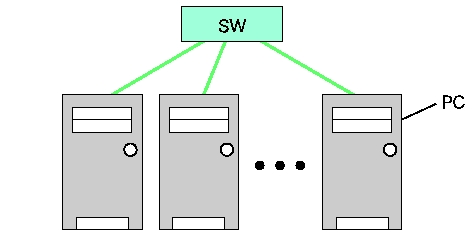
\includegraphics[width=82mm]{image200802/cluster.png}
  \caption{$B%/%i%9%?$N35G0?^(B}
  \label{fig:ga-map}
 \end{center}
\end{figure}
\vspace{-3mm}

\subsubsection{PC$B%/%i%9%?$r$D$/$kM}M3(B}
$B9bB.$J7W;;5!4D6-$,M_$7$$$1$I!"%9!<%Q!<%3%s%T%e!<%?$_$?$$$J9b2A$J@lMQJBNs7W;;5!$O$H$F$bGc$($J$$!#(B
$B$=$3$G!"IaDL$NEE5$20$GGd$C$F$$$k$h$&$J(BPC $B$r%/%i%9%?2=$7$F!"0B2A$KJBNs7W;;4D6-$r:n$m$&!"$H$$$&$3$H$,9M$($i$l$^$7$?!#(B

PC$B%/%i%9%?$K$OBg$-$/J,$1$F!"(BHA$B!J(BHigh Availability$B!K%/%i%9%?$H(BHPC$B!J(BHigh Performance Computing$B!K%/%i%9%?$,$"$j$^$9!#(B
HA$B%/%i%9%?$H$O!"9b2DMQ@-$r;}$D%7%9%F%`!"$D$^$j%5!<%S%9$r;_$^$j$K$/$/$9$k$3$H$rL\E*$H$7$?%/%i%9%?%7%9%F%`$G$9!#(B
$B:G6a$O(BWeb$B7O$N%5!<%P$G$3$N%7%9%F%`$,$h$/MQ$$$i$l$F$$$^$9!#(B
HPC$B%/%i%9%?$H$O!"2J3X7W;;J,Ln$J$I$G$*$$$F!"$b$N$9$4$/;~4V$N$+$+$k=hM}$r!"J#?tBf$N(BPC$B$KJ,;6$5$;$F!"(B
$B9bB.$K7k2L$rF@$k$3$H$rL\E*$H$7$?%/%i%9%?%7%9%F%`$G$9!#(B
$B4k6H$N%a!<%+$G$b!"<VBN$d9R6u5!$r@_7W$9$k:]$N%7%_%e%l!<%7%g%s$J$I$KMQ$$$i$l$F$$$^$9!#(B

$BK\;qNA$H%W%l%<%s$G$O4pK\E*$K(BHPC$B%/%i%9%?$K$D$$$F$NOC$G$9$,!"(BHA$B%/%i%9%?$K6&DL$7$F$$$kE@$bB?$$$O$:$G$9!#(B

\subsubsection{Debian$B$G(BPC$B%/%i%9%?$r:n$kM}M3(B}
\begin{itemize}
\item Debian$B$K$O?tB?$/$N(BPC$B%/%i%9%?MQ%D!<%k$,$"$k(B
\item PC$B%/%i%9%?$N(BOS$B$H$7$FIaDL$N(BDebian$B$rMxMQ$9$k$N$G!"(BPC$B%/%i%9%?%D!<%k0J30$NM-MQ$J%D!<%k$b?tB?$/MxMQ$G$-$k(B
\item $B%3%_%e%K%F%#$,3hH/!J(Bdebian-users$B$G<ALd$KEz$($F$/$l$k?MC#$OAG@2$i$7$$!K(B
\item apt$B$,3Z(B
\end{itemize}

\subsection{PC$B%/%i%9%?$N:n$jJ}(B}
$BJBNs7W;;$,$G$-$k$^$G$rL\I8$H$7$F!"(BPC$B%/%i%9%?%7%9%F%`$r%;%C%H%"%C%W$9$k<j=g$r@bL@$7$^$9!#(B
\begin{enumerate}
\item PC$B%/%i%9%?$r9=@.$9$kItIJ!J(BPC$B!"(BLAN$B%1!<%V%k!"%9%$%C%A%s%0%O%V!K$rMQ0U$7!"$=$l$>$l@\B3$9$k(B
\item $BMQ0U$7$?(BPC$B$K(BDebian GNU/Linux$B$r%$%s%9%H!<%k$9$k(B
\item $B<+J,$,I,MW$H$9$k%3%s%Q%$%i$HJBNs7W;;%i%$%V%i%j$r%$%s%9%H!<%k$9$k!#(B
      $BJBNs7W;;%i%$%V%i%j$O(Bmpich$B$H(BPVM$B$,$h$/MQ$$$i$l$k!#(B
      $B:#2s$O(Bmpich$B$r;H$&(B
\begin{commandline}
 # aptitude install mpich-bin libmpich1.0-dev gcc g77 g++
\end{commandline}
      $B%$%s%9%H!<%k8e$KJBNs7W;;$KMQ$$$k%[%9%HL>!J$b$7$/$O(BIP$B%"%I%l%9!K$r(B
      /etc/mpich/machines.LINUX$B5-=R$9$k(B
\item $B%/%i%9%?Fb%M%C%H%o!<%/$G$O!"B.EY=E;k$N$?$a0E9f2=$J$7$GDL?.$r9T$$$?(B
      $B$$$N$G!"(Brsh-server$B$H(Brsh-client$B$r%$%s%9%H!<%k$9$k(B
\begin{commandline}
 # aptitude install rsh-server rsh-client
\end{commandline}
      $B%$%s%9%H!<%k8e$K(Brsh$B$r5v2D$9$k%[%9%HL>!J$b$7$/$O(BIP$B%"%I%l%9!K$r(B
      /etc/hosts.equiv$B$K5-=R$9$k(B
\item NFS$B$r;H$C$F(B/home$B0J2<$N6&M-$r9T$&$HJXMx$J$?$a!"(BPC$B%/%i%9%?$r9=@.$9$k(B
      PC$B$N(B1$BBf$K(Bnfs-kernel-server$B$r%$%s%9%H!<%k$9$k(B
\begin{commandline}
 # aptitude install nfs-kernel-server
\end{commandline}
      $B$=$7$F!"(Bnfs-kernel-server$B$r%$%s%9%H!<%k$7$?(BPC$B$N(B/etc/exports$B$K!"$I(B
      $B$N(BPC$B$K(BNFS$B$N%5!<%S%9$r5v2D$9$k$+$N>pJs$r5-=R$9$k!#(B
\begin{commandline}
 $B!Z(B/etc/exports$B$NNc![(B
 /home   192.168.1.0/255.255.255.0(rw,async,no_subtree_check)
\end{commandline}
      /etc/exports$B$NJQ998e$K(BNFS$B$N%5!<%S%9$r:F5/F0$5$;$k(B
\begin{commandline}
 # /etc/init.d/nfs-kernel-server restart
\end{commandline}
      $B$=$7$F!"(Bnfs-kernel-server$B$r%$%s%9%H!<%k$7$?(BPC$B0J30$O!"(Bmount$B%3%^%s%I(B
      $B$rMQ$$$F(BNFS$B%5!<%P$K%^%&%s%H$9$k(B
\begin{commandline}
 # mount -t nfs $B!J(BNFS$B%5!<%P!K(B:/home /home
\end{commandline}
      $B0J>e$G!"(BPC$B%/%i%9%?$N40@.$G$9!#4JC1$G$9!#(B
      $B0U30$+$b$7$l$^$;$s$,!"JBNs7W;;%i%$%V%i%j0J30$OFC<l$J%=%U%H%&%'%"$rMQ$$$F$$$^$;$s!#(B
      $B$3$N$h$&$K4{B8$N%=%U%H%&%'%"$rM-8z3hMQ$G$-$k=j$,!"(BPC$B%/%i%9%?$NBg$-$JFCD'$G$9!#(B
 \item $BJBNs7W;;MQ%5%s%W%k%U%!%$%k$,!"(B
       /usr/share/doc/libmpich1.0-dev/examples/cpi.c$B$K$"$k$N$G!"<B9T$7$F(B
       $B$_$^$7$g$&!#(B
\begin{commandline}
 $ mpicc cpi.c -o pi $B!Z%3%s%Q%$%k![(B
 $ mpirun -np 5 pi   $B!Z<B9T![(B
\end{commandline}
       cpi.c$B$O(B$\pi$$B$NCM$r7W;;$9$k%W%m%0%i%`$G$9!#(B
       mpicc$B$H$$$&%3%^%s%I$G(BC$B8@8l$G=q$+$l$?JBNs7W;;%W%m%0%i%`$N%3%s%Q%$%k$,9T$($^$9!#(B
       Fortran$B$N>l9g$O(Bmpif77$B!"(BC++$B$N>l9g$O(Bmpicxx$B$J$I$rMQ$$$^$9!#(B

       $B$=$7$F!"(Bmpirun$B$H$$$&%3%^%s%I$G!"JBNs7W;;%W%m%0%i%`$N<B9T$,9T$($^$9!#(B
       $B0z?t$N(B-np$B0J9_$O%W%m%;%9?t$r;XDj$7$F$$$^$9!#(B
       $B$^$?!"JBNs7W;;$K;HMQ$7$?$$%^%7%s$r;XDj$9$k:]$O!"(B-machinefile$B$H$$$&%*%W%7%g%s$rMxMQ$7$^$9!#(B

\begin{commandline}
 $ mpirun -np 5 -machinefile hoge.txt pi
\end{commandline}

       $B$3$N>l9g!"(Bhoge.txt$B$KJBNs7W;;$K;HMQ$7$?$$%[%9%HL>$r=q$/$H!"$=$N(BPC
       $B$GJBNs7W;;$,9T$o$l$^$9!#(B
\end{enumerate}

\subsection{$B%/%i%9%?$G;H$&$HJXMx$J%=%U%H%&%'%"(B}
Ganglia$B$H$$$&3F%N!<%I$NIi2Y!"@8;`$r(BWeb$B%V%i%&%6$+$i3NG'$G$-$k%=%U%H%&%'%"!#(B
$BF|!"=5!"7n!"G/$H$$$C$?C10L$G%/%i%9%?A4BN$N%m!<%I%"%Y%l!<%8$N798~$b8+$k$3$H$,$G$-$^$9!#(B

\begin{figure}[htbp]
 \begin{center}
  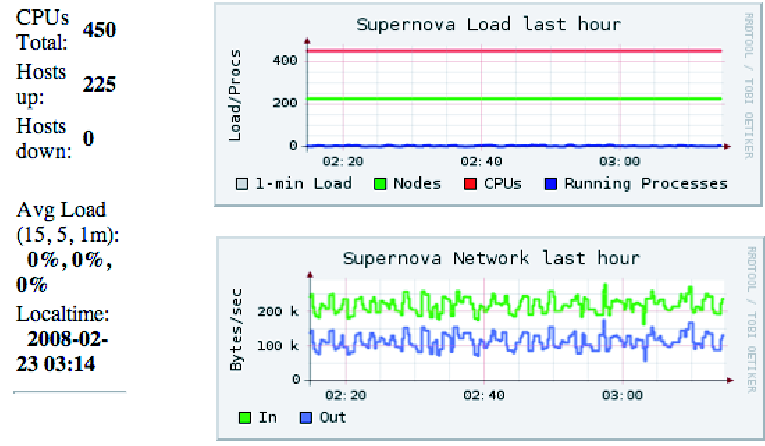
\includegraphics[width=100mm]{image200802/ganglia.png}
  \caption{Ganglia}
  \label{fig:ga-map}
 \end{center}
\end{figure}

\subsection{$B$*$o$j$K(B}
$B6n$1B-$G%/%i%9%?$N35MW$H%;%C%H%"%C%W<j=g$K$D$$$F@bL@$7$^$7$?!#(B
Debian$B$G%/%i%9%?$r:n$k$N$O4JC1$@$H$$$&$N$,EA$o$l$P9,$$$G$9!#(B

\subsection{$B;29MJ88%(B}
\begin{itemize}
\item $BF1;V<RBg3XCNE*%7%9%F%`%G%6%$%s8&5f<<!J(B\url{http://mikilab.doshisha.ac.jp/}$B!K(B
\item $BD6JBNs7W;;8&5f2q!J(B\url{http://www.is.doshisha.ac.jp/SMPP/}$B!K(B
\end{itemize}


\dancersection{$B;qNA:n@.4pAC(B(TeX)}{$B;32<(B $BB:Li(B}

\subsection{$B%$%s%9%H!<%k(B}
$B:#2s!"BP>]$H$9$k$b$N$O(B2008$BG/(B2$B7n(B21$BF|8=:_$N(Bstable$B$G$"$k(Betch$B$rBP>]$H$7$^$9!#(B
$B;d$N%;%C%7%g%s$G$O:G>.8B$N;v$7$+=R$Y$J$$$?$a!"(BYaTeX$B$J$I$r3hMQ$7$?$$J}$O!"(B
$B4XO"(BURL$B$dEl5~%(%j%"(B Debian $BJY6/2q(B2007$BG/(B12$B7n$N;qNA(B\footnote{whizzytex$B$J$I(B
$B$rMQ$$$F%W%l%S%e!<$5$;$k$J$I?'!9$H5;$,:\$C$F$$$^$9!#(B}$B$r$4Mw2<$5$$!#(B

\subsubsection{/etc/apt/sources.list$B$N3NG'(B}

$B%N%s%U%j!<$J$b$N$b;H$&$?$a!"(B/etc/apt/sources.list$B$O0J2<$N$h$&$K$7$F$*$$(B
$B$F2<$5$$!#(B

\begin{commandline}
deb http://ftp.debian.or.jp/debian/ etch main contrib non-free
\end{commandline}

\subsubsection{teTeX $B$H(B pTeX$B0l<0$N%$%s%9%H!<%k(B}
\begin{commandline}
 $ sudo aptitude install ptex-bin
\end{commandline}

\subsubsection{$B1|B<$5$s$N?7%/%i%9%U%!%$%k$N%$%s%9%H!<%k(B}
\begin{commandline}
 $ sudo aptitude install okumura-clsfiles
\end{commandline}

\subsubsection{dvipdfmx$B$N%$%s%9%H!<%k(B}
\begin{commandline}
 $ sudo aptitude install dvipdfmx
\end{commandline}

\subsubsection{Adobe Reader$B$N%$%s%9%H!<%k(B}
Etch$B$N(BEvince$B$K$OF|K\8l$N%U%)%s%H$rKd$a9~$s$G$J$$>l9g$KJ8;z$,2=$1$k$H8@$&%P%0(B 
\footnote{$B$$$/$d$5$s$,=$@5$7$?$b$N$rG[I[$7$F$$$^$9!#(B
\url{http://ikuya.info/wiki/index.php?etchpackages} 
$B$?$@!"(B2008$BG/(B2$B7n(B22$BF|8=:_$N(Bunstable$B$G$b!"(BEvince$B$K$O!"(Bpoppler$B$NLdBj$,$"$j!"(B
 \url{http://lists.debian.or.jp/debian-devel/200712/msg00000.html}$B$3$l$O!"(B
Adobe$B$H$N(BCMAP$BLdBj$K7R$,$k$N$G!"(B
Adobe Reader$B$G8+$k;v$r$*4+$a$7$^$9!#(B
}
$B$,$"$k$N$G!"(BPDF$B$r8+$k$?$a$K(BAdobe Reader$B$r%$%s%9%H!<%k$9$k!#(B

Adobe Reader$B$NG[I[%Z!<%8(B
\footnote{\url{http://www.adobe.com/jp/products/acrobat/readstep2.html}}
$B$K%"%/%;%9$7!"(BAdobe Reader$B$N(Bdeb$B%Q%C%1!<%8$r<h$C$F$/$k!#(B

\begin{commandline}
 $ sudo dpkg -i AdobeReader_jpn-8.1.2-1.i386.deb
\end{commandline}

\subsubsection{CMAP$B$N%$%s%9%H!<%k(B}
\begin{commandline}
 $ sudo aptitude install cmap-adobe-japan1 cmap-adobe-japan2
\end{commandline}

\subsubsection{YaTeX($BLnD;(B)$B$N%$%s%9%H!<%k(B}

$B%(%G%#%?$H$7$F(BEmacs$B$r;H$C$F$$$k?M$O!"(BYaTeX$B$H8F$P$l$k(B
\LaTeX $BF~NO;Y1g4D6-$,$"$k$N$G!"$=$l$rMxMQ$9$l$PNI$$$G$7$g$&!#(B
\footnote{Emacs$B$r;H$C$F$$$J$$J}$G$b!"(BVIM-\LaTeX
(\url{http://vim-latex.sourceforge.net/})$B$d(B
KDE$B4D6-$K(BKile(\url{http://kile.sourceforge.net/})$B$H$$$&(B
\LaTeX $B$rJT=8$9$k4D6-$,$"$k$h$&$G$9!#(B
}

\begin{commandline}
 $ sudo aptitude install yatex emacs21
\end{commandline}

$BJ8;z%3!<%I$O(B iso-2022-jp $B$GE}0l$7$F$$$^$9(B\footnote{Windows $BHG$H(B Linux $BHG(B
$B$N(B ptex $B$G6&DL$7$F07$($kJ8;z%3!<%I$K$7$?$H$$$&7P0^$,$"$j$^$9!#$?$@$78=>u(B
Windows $B$GA4It$G$-$k>u67$G$O$"$j$^$;$s!#(B}$B!#$?$H$($P!"(Bemacs + yatex $B$r;HMQ(B
$B$7$F$$$k>l9g$G(B iso-2022-jp $B$r%G%U%)%k%H$K$9$k$K$O!"2<5-$N$h$&$J@_Dj$r(B
\texttt{.emacs} $B$K$+$1$P$h$$$G$7$g$&!#(B

\begin{commandline}
(add-hook 'yatex-mode-hook
	  '(lambda () 
	     (progn 
	       (if (string-match "^/home/user/monthly-report/" default-directory)
		   (progn (set-buffer-file-coding-system 'iso-2022-jp)
			  (set-buffer-modified-p nil))))))
\end{commandline}

\texttt{.emacs}$B$NNc$G$9!#(B

\begin{commandline}
;;;;;;;;;;;;;;;;;;;;;;;;;;;;;;;;;;;;;;;;;;;;;;;;;;;;;;;;;;;;;;;;;;;;;;;;;
;; YaTeX
;;;;;;;;;;;;;;;;;;;;;;;;;;;;;;;;;;;;;;;;;;;;;;;;;;;;;;;;;;;;;;;;;;;;;;;;;
(setq auto-mode-alist
      (cons (cons "\\.tex$" 'yatex-mode) auto-mode-alist))
(autoload 'yatex-mode "yatex" "Yet Another LaTeX mode" t)
(defvar YaTeX-dvi2-command-ext-alist
  '(("xdvi" . ".dvi")
    ("ghostview\\|gv" . ".ps")
    ("acroread" . ".pdf")))
 (setq dvi2-command "acroread")
(setq dviprint-command-format "dvipdfmx `basename %s pdf`dvi")
;;; $B?'IU$1(B
(setq YaTeX-use-font-lock t)
(add-hook 'yatex-mode-hook
	  '(lambda () 
	     (progn 
	       (if (string-match "^/home/user/monthly-report/" default-directory)
		   (progn (set-buffer-file-coding-system 'iso-2022-jp)
			  (set-buffer-modified-p nil))))))
\end{commandline}

\subsection{$BJ8>O$NJT=8(B}

\LaTeX $B$O:G=i$OFq$7$$$H46$8$k$+$b$7$l$^$;$s$,!"4pK\$O(B HTML $B$H;w$?$h$&$J(B
$B$b$N$J$N$G!"$^$:$O%=!<%9$rFI$`;v$+$i;O$a$F$_$k$HNI$$$+$b$7$l$^$;$s!#(B
\LaTeX $B$K$D$$$F$5$i$KCN$j$?$$J}$O!"(B
$B!V(B[$B2~D{Bh(B4$BHG(B] \LaTeX 2$BH~J8=q:n@.F~Lg(B
($BBg7?K\(B)$B!!1|B<(B $B@2I'(B ($BCx(B) $B!W(B
$B$J$I$NK\$rFI$`;v$r$*4+$a$7$^$9!#(B

\subsubsection{$B%j%]%8%H%j$+$i%G!<%?$r<h$C$F$/$k(B}
$B8=:_!"4X@>(B Debian $BJY6/2q$G$O!"%j%]%8%H%j$NMQ0U$,=PMh$F$$$J$$$?$a!"(B
$BEl5~%(%j%"(B Debian $BJY6/2q$N%j%]%8%H%j$r<Z$j$F$$$k>uBV$G$9!#(B

\begin{commandline}
 $ sudo aptitude install git-core
 $ git-clone git://git.debian.org/git/tokyodebian/monthly-report.git
\end{commandline}

$B%I%-%e%a%s%H$O(B p\LaTeX{}$B$G:n@.$7$F$$$^$9!#%U%!%$%kL>$H$7$F2<5-$K$J$C$F$$(B
$B$^$9!#(B(YYYY)(MM)$B$O!"G/$H7n$G!"Nc$($P(B2008$BG/(B02$B7n$G$"$l$P(B 200802 $B$G$9!#(B

\begin{description}
 \item[debianmeetingresume(YYYY)(MM)-kansai.tex]
	    $B;vA0G[I[;qNA(B
 \item[debianmeetingresume(YYYY)(MM)-kansai-presentation.tex]
	    $B%W%l%<%s%F!<%7%g%sMQ(B (prosper$B$rMxMQ(B)
 \item[image(YYYY)(MM)/]
	    $B2hA|%U%!%$%k$J$I$NCV$->l(B
\end{description}

\subsubsection{$B4pK\ItJ,$N@bL@(B}

$B%9%?%$%k%U%!%$%k$O(B kansaimonthlyreport.sty $B%Q%C%1!<%8$rMxMQ$7$^$9!#(B
$B$3$N%9%?%$%k%U%!%$%k$O!"El5~%(%j%"(B Debian $BJY6/2q$N%9%?%$%k%U%!%$%k$,(B
$B%+%i!<$J$N$G!"%b%N%/%m$G$b8+$d$9$$$h$&$KJT=8$7$^$7$?!#(B
$B:#8e!"$$$m$$$m$H<j$r2C$($F$$$/$H;W$$$^$9!#(B

\begin{commandline}
\usepackage{kansaimonthlyreport} 
\end{commandline}

$B3FC4EvItJ,$O(B section $B$H$7$F07$$$^$9!#FCJL$J%3%^%s%I(B dancersection $B$G;XDj(B
$B$7$^$9!#7A<0$O(B \texttt{dancersecion\{$B%?%$%H%k(B\}\{$B:n<TL>(B\}}$B$G$9!#(B
$B$=$NCf$G(B subsection $B$d(B subsubsection $B$rMxMQ$7$FJ8=q$r9=@.$7$F$/$@$5(B
$B$$!#(B

\begin{commandline}
 \dancersection{Debian $BJY6/2q;qNA$N=`Hw$NJ}K!(B}{$B>e@n(B $B=c0l(B}
 \label{sec:debmtg2007howtoprepare}
\end{commandline}

$B3FC4EvItJ,$O(B section $B$H$7$F07$$$^$9!#FCJL$J%3%^%s%I(B dancersection $B$G;XDj(B
$B$7$^$9!#7A<0$O(B \texttt{dancersecion\{$B%?%$%H%k(B\}\{$B:n<TL>(B\}}$B$G$9!#(B
$B$=$NCf$G(B subsection $B$d(B subsubsection $B$rMxMQ$7$FJ8=q$r9=@.$7$F$/$@$5(B
$B$$!#(B

\begin{commandline}
 \dancersection{Debian $BJY6/2q;qNA$N=`Hw$NJ}K!(B}{$B>e@n(B $B=c0l(B}
 \label{sec:debmtg2007howtoprepare}
\end{commandline}

\subsubsection{$B2hA|%U%!%$%k$N=hM}(B}

$B2hLL<L??$N2hA|$rDI2C$9$k$H$-$O!"$G$-$k$@$1%5%$%:$N>.$5$$(B png $B$J$I$rMxMQ(B
$B$7$F$/$@$5$$!#%0%i%U$J$I$N@~2h$G$"$l$P!"(Beps$B$G$+$^$$$^$;$s!#(Bpng $B$G$"$l$P!"(B 
ebb $B%3%^%s%I$rMxMQ$7$F(Bbounding box $B$r:n@.$7$F$/$@$5$$!#(B

\begin{commandline}
 ebb XXX.png
\end{commandline}

$B$=$7$F<!$N$h$&$K$7$FJ8>O$KKd$a9~$_$^$9!#(B

\begin{commandline}
\begin{figure}[!htbp]
\begin{center}
 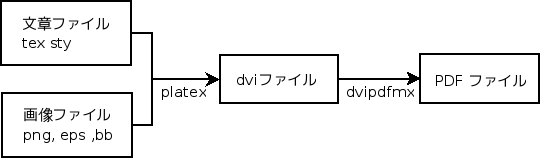
\includegraphics[width=120mm]{image200802/latex.png}
 \caption{\LaTeX $B$GJQ49$9$k%$%a!<%8(B}
 \label{fig:latex}
\end{center}
\end{figure}
\end{commandline}

\subsection{PDF$B$X$NJQ49(B}

$BJQ49$N2aDx$r4JC1$J?^$G<($9$H!"?^(B\ref{fig:latex}$B$N$h$&$K$J$j$^$9!#(B

\begin{figure}[!htbp]
\begin{center}
 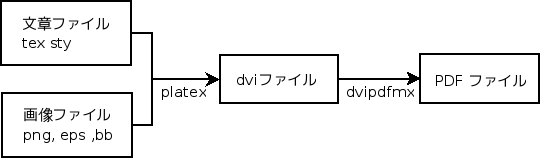
\includegraphics[width=120mm]{image200802/latex.png}
 \caption{\LaTeX $B$GJQ49$9$k%$%a!<%8(B}
 \label{fig:latex}
\end{center}
\end{figure}

$B%3%^%s%I$G0l$D$:$DJQ49$r$9$k$J$i$P!"(B
\begin{commandline}
 $ platex debianmeetingresume200802-kansai.tex
 $ dvipdfmx debianmeetingresume200802-kansai.dvi
\end{commandline}

$B$G$9$,!"%j%]%8%H%j$+$iF~<j$7$?$b$N$G$"$l$P!"(B

\begin{commandline}
 $ make
\end{commandline}

\texttt{make}$B%3%^%s%I$@$1$G%U%!%$%k$N99?7$,$"$C$?%U%!%$%k$NJQ49$J$I$r(B
$B9T$J$C$F$/$l$^$9!#(B

\dancersection{$B:#8e$NM=Dj(B}{$B;32<(B $BB:Li(B}

\subsection{$B<!2s(B}
$B<!2s$O!"(B2008$BG/(B03$B7n(B23$BF|$K:#2s$HF1$8$/(B
$B9A6hL1%;%s%?!<(B\footnote{\url{http://www.city.osaka.jp/shimin/shisetu/01/minato.html}}
$BG_$K$F9T$J$$$^$9!#(B

\subsection{OSC Kansai$B$K$D$$$F(B}
$B:#G/$N(BOSC Kansai$B$NF|Dx$,7h$^$j$^$7$?!#(B
7$B7n(B18,19$BF|!J6b!&EZ!K$K9T$J$o$l$^$9!#(B

3$B7n$NCf=\:"!"(BOSC Kansai$B$N%-%C%/%*%U%_!<%F%#%s%0$,$"$k$N$G!"(B
$B4X@>(B Debian $BJY6/2q$b4X78<T$,;22C$7!">\$7$$OC$rJ9$$$F$-$^$9!#(B

\subsection{KDR$B$N$*$7$i$;(B}
$B4X@>(BDebian$BJY6/2q$NM-;V$G(B
$B4X@>(BDebian$BJY6/2q$H$OFHN)$7$?7A$G!"(B
$B=5$K0lEY!"FI=q2q(B(KDR)$B$r3+$$$F$$$^$9!#(B
$B>\$7$/$O(B\url{http://qwik.jp/kdrweb/}$B$r$4Mw2<$5$$!#(B
$B!!(B
\printindex
 \cleartooddpage

 \begin{minipage}[b]{0.2\hsize}
  \rotatebox{90}{\fontsize{80}{80} {\gt $B4X@>%G%S%"%sJY6/2q(B} }
 \end{minipage}
 \begin{minipage}[b]{0.8\hsize}

 \vspace*{15cm}
 \rule{\hsize}{1mm}
 \vspace{2mm}
 
\includegraphics[width=2cm]{image200502/openlogo-nd.eps}
 \noindent \Large \bf Debian $BJY6/2q;qNA(B\\ \\
 \noindent \normalfont \debmtgyear{}$BG/(B\debmtgmonth{}$B7n(B\debmtgdate{}$BF|(B \hspace{5mm}  $B=iHGBh(B1$B:~H/9T(B\\
 \noindent \normalfont $B4X@>(B Debian $BJY6/2q(B $B!JJT=8!&0u:~!&H/9T!K(B\\
 \rule{\hsize}{1mm}
 \end{minipage}

\end{document}
